\capitulo{4}{Técnicas y herramientas}

Apartado cuyo objetivo es presentar las técnicas metodológicas y las herramientas de desarrollo que se han utilizado para llevar a cabo el proyecto. Si se han estudiado diferentes alternativas de metodologías, herramientas, bibliotecas, etcétera.\\

Se comenta los aspectos más destacados de cada opción, con un repaso somero a los fundamentos esenciales y referencias bibliográficas para que el lector pueda ampliar su conocimiento sobre el tema.
\section{¿Por qué Python?}
La razón es la sencillez y capacidad de este lenguaje para el análisis y tratamiento de los datos gracias a librerías como Pandas o Numpy. Base gran parte de la metodología de análisis usada en este proyecto en el libro: Python for Data Analysis. \cite{pythonDataAnalisis}
\\ 
Las distintas posibilidades que se barajaron antes de empezar fueron Java, Android, R y Python. Al final me decanté por Python por diferentes motivos, el primero en ser descartado fue Java, tras un estudio inicial sobre lo que quería hacer y el como hacerlo, me di cuenta que necesitaba un lenguaje potente que me dejase tratar los datos con claridad para su análisis, y después de leer varios artículos como: REFERENCIA ARTICULOS, me percaté de que Java no era la mejor opción, estos artículos siempre te orientaban hacia Python y R. Entonces, ¿Por qué Android?, por la sencilla razón de que este trabajo está desarrollado para unir el mundo de la dietoterapia, y las ciencias de la Salud con la informática para hacer que el usuario tenga un fácil aprendizaje de dicha metodología. A mi parecer la forma más clara y rápida de llevar al usuario dicha tecnología es a través de su SmartPhone, pero se acabó descartando debido a la falta de conocimientos sobre sistemas Android. A estas alturas ya solo me quedaba elegir entre Python y R, tras indagar superficialmente sobre ambos lenguajes para el análisis y el tratamiento de datos, se llego a la conclusión que ambos lenguajes tienen una forma de trabajar muy similares, y entonces la decisión fue clara, debido a que he trabajado en numerosas ocasiones con Python y la sintaxis de R para mi era desconocida, al final, me decante por Python.
\section{Metodología}
\subsection{Introduccón}
En este apartado explicaremos el cómo y porque se ha tratado los datos en este TFG además de los diferentes cálculos internos que se realizan para el sistema de recomendaciones, cálculos, etc.
\subsection{Excell y Pandas}
Se ha usado la herramienta de Microsoft Excel, para trabajar como una base de datos, trabajando los datos en formato DataFrame. Los DataFrame son proporcionados por la librería Pandas. Hay un Excel para la base de datos genérica,otro para la base de históricos y otro para los usuarios. Se leen los datos automáticamente en cuanto el usuario entra en la aplicación, pero solo se guarda si el usuario así lo desea.
\subsection{DataFrame}
Se usan los DataFrame, para llevar un registro de todos los datos que el programa necesita, se tiene en cuenta tanto las bases de datos de los alimentos, usuarios y comidas como lo que el usuario lleva en el día.
\\
Los alimentos se tratan en el momento en el que se registra el usuario, de manera que, se separan las comidas de la lista principal, creando 5 listas (Desayuno, Merienda, Comida, Almuerzo y Cena), se tratan por separado y se filtran. Cada modificación o inserción de un dato o usuario se hace sobre el DataFrame, el cual sustituirá a la base de datos durante el guardado.

\section{Técnicas}
\subsubsection{Introducción}
En este apartado se hablara brevemente de las técnicas usadas durante el proyecto, y la razón por la que se escogieron dichas técnicas. Posiblemente, haya argumentos repetidos en otros apartados similares, por ello se expresará exclusivamente finalidad y razonamiento.
\subsection{Aprender a aprender}
\begin{quote}
“Aprender a aprender supone disponer de habilidades para iniciarse en el aprendizaje y ser capaz de continuar aprendiendo de manera cada vez más eficaz y autónoma de acuerdo a los propios objetivos y necesidades.\\

Esta competencia tiene dos dimensiones fundamentales. Por un lado, la adquisición de la conciencia de las propias capacidades (intelectuales, emocionales, físicas), del proceso y las estrategias necesarias para desarrollarlas, así como de lo que se puede hacer por uno mismo y de lo que se puede hacer con ayuda de otras personas o recursos. Por otro lado, disponer de un sentimiento de competencia personal, que redunda en la motivación, la confianza en uno mismo y el gusto por aprender. Significa ser consciente de lo que se sabe y de lo que es necesario aprender”. \cite{aprederAAprender}


\end{quote}

Es decir, el auto-aprendizaje no solo ayuda al usuario a aprender de manera autónoma, sino que le ayuda, a que todo aquello que ha conseguido, para el sea, de alguna forma, una meta, algo que lograr, algo suyo, que no se le va a olvidar tan fácilmente, como información memorizada, sino que será el resultado de pequeños logros personales que integrarán al usuario, una nueva información, como si fuese suya.
\subsection{TMB}
Se traduce como el calculo o tasa del metabolismo basal, por si no lo recuerdan, el metabolismo basal, es el gasto calórico que llevamos a cabo en reposo, por el mero hecho de respirar, a este calculo se le suman una serie de variables relacionadas con la actividad física del usuario y como resultado tenemos las kilocalorías diarias que el usuario gasta al día o que es equivalente que el usuario debe tomar para mantenerse en su peso, obviamente, este calculo es genérico, es muy utilizado por endocrinos, cuya finalidad no es hacer un seguimiento estricto de una dieta, sino un calculo aproximado de esta, para la correcta alimentación del paciente.\\

Tras horas de estudio, se aproximó que la forma mas correcta de bajar o subir peso en base al cálculo del metabolismo basal, es dar un margen de 500 kilocalorías, arriba o abajo, según los propósitos de nuestro usuario. Se recalca, que es claro que es un cálculo genérico pero hasta el perfeccionamiento del proyecto, es el calculo mas adecuado que podemos realizar. Dicho calculo se sustenta a través de la siguiente formula:
\textbf{Hombres:}
\begin{equation}
TMB =  ((10 * Peso(kg))+(6,25*Altura (cm))-(5*edad)+5)*ActividadFisica
\end{equation}
\textbf{Mujeres:}
\begin{equation}
TMB =  ((10 * Peso(kg))+(6,25*Altura (cm))-(5*edad)-161)*ActividadFisica
\end{equation}
Donde actividad física se corresponde con los siguientes valores mostrados en la Tabla 4.3. \cite{TMB}
\tablaSmall{Valor de la actividad física en TMB}{l c c c c}{TablaActividadYMB}
{ \multicolumn{1}{l}{Ejercicio } & Valor de ActividadFisica\\}{ 
Poco ejercicio & 1,2\\
Ejercicio ligero(1-3 dias/semana) & 1,35\\
Ejercicio Moderado (3-5 diás/semana) & 1,55\\
Ejercicio fuerte (6-7 dias/semana & 1,725\\
Ejercicio muy fuerte (dos veces al día) & 1,9 \\
} 
\subsection{Tratamiento de Excepciones}
A través del tratamiento de excepciones, y con el uso de la librería \textbf{messagebox} se informa al usuario de las distintas situaciones que se pueden dar durante el uso del programa. Existe tres tipos principales de cuadros de textos, que emergen informando al usuario de algún tipo de problemao simplemente de que una acción ha finalizado correctamente.\\


\textbf{Información}\\

\begin{figure}[h]
\centering
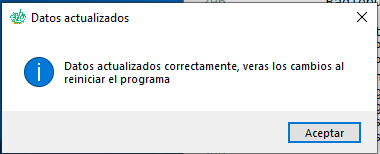
\includegraphics[scale=1]{Informacion} 
\caption{Ventana emergente de información}
\end{figure}
Muestra la información de que un proceso a concluido correctamente. También explican si el usuario ha de realizar algo una vez terminado el proceso para que termine la completa finalización de este.\\


\textbf{Aviso}\\

\begin{figure}[ht]
\centering
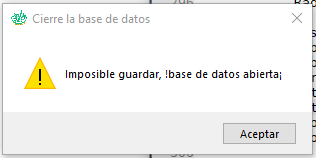
\includegraphics[scale=1]{Aviso} 
\caption{Ventana emergente que avisa que una acción no se ha podido realizar.}
\end{figure}
Pantalla que advierte que algo no ha salido bien. El usuario puede seguir con el uso del programa, pero si quiere realizar la acción que estaba realizando, deberá seguir las instrucciones proporcionadas en el cuadro de aviso.\\

\textbf{Error}\\

\begin{figure}[ht]
\centering
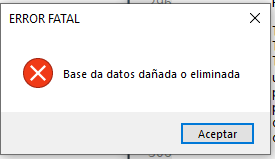
\includegraphics[scale=1]{Error} 
\caption{Ventana emergente que muestra que ha ocurrido un Error.}
\end{figure}
Pantalla que advierte de un Error grave, en el que se ha corrompido la estructura de datos del programa.\\

A través de estos cuadros se traduce los diferentes problemas que puedan surgir en la utilización del programa; de manera gráfica y entendible por el usuario, haciendo el funcionamiento de este lo más transparente al usuario posible.
\section{Estructura del programa}
\subsection{Introducción}
En un principio se pensó en hacer una estructura MVC clásica pero conforme el proyecto fue creciendo, y prácticamente de manera imperceptible se convirtió en una versión un tanto modificada de este modelo.\\

La estructura se basa en cuatro módulos principales, además de las librerías pertinentes, obviamente. 
\begin{enumerate}
\item	\textbf{Main} – Tronco del programa
\item	\textbf{Vistas} – Relacionado con la parte visual
\item	\textbf{CalculosDieta} – Todo calculo usado en el programa
\item	\textbf{AdminBase} – Todo proceso relacionado con la base de datos

\end{enumerate}
En los apartados siguientes se hablará de manera extensa sobre las librerías utilizadas y los módulos creados para el desarrollo
 de esta aplicación, por el momento, este apartado será explicando en que deriva y se basa dicha estructura, conforme el MVC clásico y cuales son las consecuencias de esto.
\subsection{Cálculos, Administración y vista}
Podríamos llamar propiamente a este modelo el CAV, y se basa en separar toda función que se vaya a crear en el programa en estos tres pilares. \\
Todo surgió de la necesidad de separar la administración de la base de datos con cualquier otro tipo de función en el programa, esto sin darme cuenta creaba una cuarta pata en el trípode que supone el MVC. Este fue uno de los motivos, pero el motivo principal fue menos precipitado, se iba creando un módulo cada vez que la lógica de una función necesitará un hueco donde encajar y ninguno de los módulos creados lo sostenía. Debido a mi forma de trabajar, me sentí cómodo de dividirlo así, creando inicialmente una estructura básica y modulada, pero no en exceso. Por un lado, todo elemento relacionado con la base de datos, por otro lado todo cálculo matemático realizado en el programa y por ultimo toda función que intervenga en la interacción usuario-aplicación.\\

Esto tuvo en su momento sus inconvenientes, surgían funciones que encajaban en diferentes módulos debido a que igual era puramente visual, pero interactuaba con la base de datos, o llevaba a cabo unos cálculos para dibujártelos visualmente, por ello se llevo a cabo una serie de reglas sencillas:
\begin{itemize}
\item	Si su finalidad es puramente visual – Vista
\item	Si realiza cálculos u operaciones matemáticas, indistintamente de si sea sobre la dieta -CalculosDieta
\item	Si interacciona y guarda datos en la base de datos -AdminBase
\item	Si mezcla alguna de estas funcionalidades, por ejemplo, guardar en la base de datos y mostrar por pantalla algo, se tendrá en cuenta cual es su principal finalidad, por ejemplo, se guardan estilos, que se cargaran automáticamente para el diseño del programa, obviamente su finalidad es puramente visual, y guardar en la base de datos una transacción necesaria.
\item	Cualquier Objeto, ventana, tabulación, etc. Que siempre vaya estar ahí al Main, pero sus modificaciones se repartirán entre los diferentes módulos.

\end{itemize}
Estas reglas, a día de hoy, han cumplido con todas las funciones que se han creado en el programa dando el resultado previsto.
\section{Librerías}
\subsection{Pandas}
La librería desarrollada por Wes McKinney, Pandas, es una librería usada para el tratamiento de los datos como estructuras. No fue la primera opción para este proyecto, debido a que este proyecto se enfoca en el análisis de datos, y no en el tratamiento de bases de datos, se decidió crea una base de datos local en un archivo Excel, la primera opción fue la librería “openpyxl”, la cual, es una librería de código abierto, que permite la carga y manejo de datos XLS, el problema vino que te devolvía objetos desestructurados difíciles de tratar, y complicaba él objetivo principal del proyecto, acto seguido basándome en él libro: LIBRO, decidí probar con Pandas, esta librería me permitía leer los datos de los archivos .XLS, en forma de dataframes. Esto simplificaba el análisis de los datos, permitiendo tratarles tanto como dataFrame como en forma de numpy.array, dicha librería será analizada a continuación.
\subsection{Numpy}
Como ya he nombrado en varias ocasiones en este memoria, el libro: LIBROO, se basa principalmente en esta librería, como añadido, es la librería sobre la que he trabajado a lo largo de la carrera en cuanto a análisis de datos en Python, y la mas recomendada por los usuarios en la web, sobre esta librería se sustenta principalmente este proyecto, siendo la encargada, del tratamiento, procesamiento y calculo, de todos los datos que internamente realiza el programa.
\subsection{Interfaz Gráfica}
La librería utilizada para realizar y diseñar la interfaz gráfica fue Tkinter, tras buscar en diferentes páginas que encontraremos en la bibliografía, me decante por Tkinter debido a la falta de conocimientos en interfaces gráficas con Python, me decante por la mas fácil de aprender. Entre las opciones que baraje se encontraban: Tkinter, WxPython, PyQt y PyGTK.\\

Tkinter traía una serie de ventajas, entre ellas que viene preinstalada con Python, era fácil de aprender, y hay una documentación amplia y extensa. Pero también tiene sus desventajas, incluye pocos elementos gráficos, tiene un limitado control y la navegabilidad mas sencilla se hace complicada, y sobre todo lo que mas noto es su lentitud, cuanto mas elementos añadas, mas lento va la interfaz, no tiene alguna especie de cache o memoria que guarde lo que has “dibujado”, sino que los dibuja cada vez que salen en pantalla, lo hace sobre cada botón etiqueta, etc.\\

La segunda opción que se me paso por la cabeza, fue WxPython,  tenia grandes ventajas, como la rapidez,  la flexibilidad que este ofrecía y sobre todo su mayor ventaja son todas las opciones que tiene para crear una interfaz gráfica compleja y “profesional”, tras barajar, estas opciones y compararlas con las de Tkinter, me di cuenta que todo lo que te ofrecía WxPython, era innecesario para la interfaz tan simplista que necesitaba para mi proyecto, y el aprendizaje era más complejo, además de ser mas complicado encontrar información o documentación sobre esta librería. El mayor problema de esta librería era que tiene una comunidad muy activa, la cual, esta constantemente insertando cambios, esto era un problema para proyectos largos, pues creaba problemas de compatibilidad, pero para este proyecto, no era algo que me resultará un inconveniente.\\

El resto de librerías fueron descartadas, al poco de buscar información sobre ellas debido a que daban las mismas ventajas o similares que la WxPython, pero tenían mas inconvenientes, al menos para el tema que aborda este proyecto.
\subsection{Diseño}
Se decidió realizar un diseño simple, sin complicaciones, ni laberintos internos de pura navegabilidad que haga del manual de usuario un mapa para guiarse a través del programa. Esta decisión trivial se llevó a cabo debido al principal objetivo del proyecto, el aprendizaje de la dietoterapia, esta aplicación esta, básicamente, orientada a todos los públicos, por lo que si se construye una aplicación tediosa, solo complicaría el uso y aprendizaje del usuario.\\

Se basa en un menú principal ramificado en tres vertientes: Usuario, Dieta y Registro (en el programa aparecen con otros nombres, pues aquí se explica la lógica del diseño). En la vertiente usuario, esta la información del usuario y la posibilidad de cambiar dichos datos para un avance del programa. En la rama de la dieta, se encuentra el tronco principal de la aplicación, se muestra las recomendaciones alimenticias, a parte de darte libertad a la hora de escoger y decidir que deseas comer en el día de hoy. Por último, estaría el registro o historial, es decir todo aquello que necesites para llevar un registro de tu progreso y concienciar de esta manera al usuario.\\

Respecto a los colores, se decido un tema básico que no agote la vista del usuario, ni tenga múltiples colores deslumbrantes, da la posibilidad al usuario de elegir entre una serie de estilos predefinidos para que escoja el que mejor se ajuste a sus gustos y necesidades.\\
\section{Módulos}
\subsection{Cálculos Dieta}
Es el modulo principal sobre el que se sustenta el programa, hace todos los cálculos de recomendación, kilocalorías, repartos, etc.\\
En el manual del programador se extenderá mas sobre cada función, a continuación, se hará un breve comentario sobre cada función en base a la metodología.
\subsubsection{CalculoTMB, rapartoDeKcal y distribuciónDeMacronutrientes}
Estas tres funciones trabajan de manera paralela, el \textbf{calculoTMB}, lo que hace es calcular el gasto calórico basal, de aquí se saca el objetivo diario, una vez calculada la cantidad de Kilocalorías diarias, se reparten las kcal (\textbf{repartoDeKcal} )según sea desayuno, almuerzo, merienda o cena, se reparten en base a unos porcentajes calculados en base a distintas fuentes de información encontrados a lo largo del estudio sobre el que se sustenta este proyecto, no son porcentajes exactos. Su distribución es plasmada en la Tabla 4.4
\tablaSmall{Porcentajes totales de cada comida}{l c c c c}{porcentajesTipoComida}
{ \multicolumn{1}{l}{Comida } & Porcentaje(\%) & Descripción\\}{ 
Desayuno & 24,75 & Alta carga calórica, rica en hidratos\\
Almuerzo & 13,5 & Baja carga calórica.\\
Comida & 30,5 & Mayor carga calórica, eje central.\\
Merienda & 11,5 & comida de paso y casi prescindible.\\
Cena & 19,75 & Alta carga calórica pero con moderación.\\
} 
A la par se calcula el número de Kilocalorías que se tiene que tomar de hidratos, grasas y proteínas, en base al tipo de dieta recomendable para tu patología en la función distribuciónDeMacronutrientes, Esta función toma como parámetros las kilocalorías diarias calculadas previamente por la función calculoTMB, y el tipo de dieta del usuario en base a su patología, y te devuelve una lista de los macronutrientes diarios, repartidos en gramos y las kilocalorías totales en el siguiente orden: ListMacDiarios [Kilocalorías, Hidratos, Proteínas, Grasas ].

\subsubsection{OrdMinimaDiferencia y  formulDif}
Antiguamente eran dos funciones, pero se prescindió de una tras comprobar que la función \textbf{OrdMinimaDiferencia}, internamente y de manera indirecta ya lo implementaba. Estas dos funciones son usadas juntas estando formulDif dentro de OrdMinimaDiferencia.\\

son el pilar base de esta aplicación, en cuanto al calculo de comidas se refiere, OrdMinimaDiferencia, coge como parámetros la lista de las comidas, el objetivo, el tipo de comida, lo que ya llevo comido y las kilocalorías diarias. En base a esto hace un calculo de lo que debería llevar de cada macronutriente concreto en cada comida concreta en el total del día(Siendo esto el sumatorio de las comidas anteriores), lo que debería llevar de cada macronutriente específico en esa comida específica, luego se recorre todas las comidas de las bases de datos calculando cual es la que mas se ajusta a lo que necesitamos, una vez cogemos la comida le pasamos todo lo calculado anteriormente, y se lo pasamos a formulDif, para llevar a cabo la fórmula, que consiste en:
\begin{equation}
DiferenciaMacronutriente = \frac{(KMCD - A)}{((KCDT-KMM)+(KMTC-KTM))}
\end{equation}
Donde:
\begin{itemize}
\item \textbf{KMCD:} Número de Kcalorias del macronutriente (Hidratos,proteinas o grasas) de la Comida (Desayuno, almuerzo...) que debería llevar en esa comida
\item \textbf{A:} Actual número de kcalorias de ese macronuetriente que llevo en todo el día (Si estoy en Comida: desayuno+almuerzo+comida).
\item \textbf{KCDT:} Kilocalorias que debería comer en esta comida concreta para este macronutriente concreto.
\item \textbf{KMM:} Kilocalorias del macronutriente concreto del menú.
\item \textbf{KMTC:} Kilocalorias totales que debería comer en esta comida.
\item \textbf{ktm:} kilocalorias totales que tiene el menú a recomendar.

\end{itemize}

De esta manera cuanto mayor sea la diferencia entre lo que debo llevar y lo que llevo, y menor sea la diferencia entre lo que deseo y las características del alimento, mayor será la puntuación de ese alimento para su recomendación ( \textbf{Nota: Se ordena de mayor diferencia a menor}).\\
Por ultimo se realiza la media entre los tres macronutrientes principales:
\begin{equation}
DiferenciaTotal = \frac{(DiferenciaHidratos+DiferenciaProteina+DiferenciaGrasas)}{3}
\end{equation} 
En el caso de que en algún macronutriente nos hallamos pasado y la diferencia de negativa, ese macronutriente no se tendrá en cuenta.
\subsubsection{Gráficos}
Hay dos tipos de gráficos por lo general, que buscan mostrar al usuario de manera clara y transparente su progreso a lo largo del uso del programa, dicho progreso se verá a través de la calidad, por ello, dividirlo en dos tipos de gráficos
Gráfico total, que hace una media de la calidad, es decir del como has comido en todo el día, del ultimo mes, y te lo muestra por pantalla, permitiéndote ver si hay mejora o no.\\

Los otros tipos de gráficos son por comida, una vez el usuario, vea su progreso general, este puedo mirar los gráficos del desayuno, comida, merienda… Así poder ver que comida le cuesta mas o menos de manera sencilla y clara.\\

\subsection{AdminBase y estructura de la base de datos}
En este apartado se expone la estructura la base de datos, y de como se cargan, se guardan y se trabajan con los datos desde el módulo AdminBase, el cual, es un modulo bastante simple, necesario para el trato de datos.
\subsubsection{CargaBaseDeDatos y guardaDatos}
Estas dos funciones cargan y guardan los datos de/en la base de datos respectivamente, como se decidió simular una base de datos con un Excel, se usa la librería Pandas, mencionada antes en este apartado para cargar las bases de datos en los respectivos arrays, nada más arrancar el programa, te guarda las tres bases de datos principales, Alimentos, usuarios, patologías e historial en cuatro vectores independientes, que se trabajaran con cada uno de ellos sin tener en cuenta al resto y se guarda el resultado de los cambios producidos durante la ejecución del programa. \\

Recordemos que estos cuatro valores se sacan de tres Excel diferentes, un Excel nombrado BaseDeDatosDeAlimentos que contiene la lista de alimentos y patologías, otro llamado BaseDeDatosUsuarios, en un principio estos dos estaban juntos, pero separarlos en dos Excel diferentes nos permite la mejor trata de datos a la hora del almacenamiento, y el historial, el cual lleva consigo un listado de las fechas y los usuarios como clave primaria, junto a todo lo que han comido ese día.\\
\subsubsection{Estructura de la base de datos}
La base de datos se estructura en dos archivos Excel independientes, donde cada hoja seria lo equivalente a una colección de una base de datos, y cada fila seria un objeto dentro de dicha colección. A distinguir las siguientes hojas:\\

\textbf{\textsc{ALIMENTOS}}\\
La hoja de alimentos, en verdad, sería una hoja de menús ya construidos los cuales tienen 10 campos, sobre los que actualmente se trabajan 8,pero se mantiene su estructura para posibles ampliaciones.\\

La clave primaria de esta colección sería el nombre, en un futuro esta pensado añadir un id, o depende la metodología de desarrollo de la base de datos, ese id se generaría de manera automática teniendo en cuenta que no sigue ningún tipo de normal en relación con el alimento.
Los campos son:
\imagen{A}{Estructura base de datos alimentos}
Nombre (PK), Calorías, Grasa, Saturadas, Hidratos,Fibra, Azucares, Proteína,Sodio, Tipo, LRE, Calidad
De los primeros siete campos no hay mucho mas que añadir, que lo que el propio nombre indica, no obstante, se hará una pequeña aclaración de los últimos tres.\\

El tipo, marca el tipo de comida que es, se pensó en que metodología usar, teniendo en cuanta que un mismo menú puede ser a la vez, desayuno, almuerzo y merienda, cena y comida, y un largo etcétera. Por ello se pensaron dos posibilidades, la primera poner la inicial, letra o nombre de la comida para la que valga ese menú, tratarlo como un array y descomponerlo en su debido momento, pero en el futuro caso de que se diera la posibilidad al usuario de editar un alimento de manera que no le apareciese entre una comida específica se complicaba algo más, y la segunda opción era tratarlo como una cadena de bits: desayuno-almuerzo-comida-merienda-cena, donde el valor 1 sería si es valido para esa comida y 0 si no lo es. Por ejemplo:\\
1-1-0-1-0 \\

Significa que es desayuno, almuerzo y merienda, pero no comida o cena, luego esto se traduce en el número decimal, que en este caso sería 26.\\

El LRE, recibe ese nombre por un juego de palabras con la gestión de procesos de un sistema operativo LRU (last reciently used), pues lo que hace es llevar una métrica de la frecuencia con la que el usuario toma esa opción, literalmente significa “last reciently eat”. \\

La Calidad, como el propio nombre indica, es la calidad del alimento, es la variable de indicar la diferencia entre 100 kilocalorías de ensalada y 100 kilocalorías de azúcar, tiene un rango de valores entre el uno y el cuatro,  siendo cuatro la peor calidad de todos, y uno por el contrario la mejor, la calidad va estrechamente relacionada con el umbral del momento y la comida dentro del programa, esta variable, empieza con el valor uno (siendo este el mas bajo posible) y según vas refrescando va aumentando para que las posibilidades de menú aumenten con el número de veces que refresques la comida. El umbral sirve para cribar del DataFrame de la comida que estemos trabajando, todos los alimentos cuya calidad sea superior al valor del umbral en el momento de selección, de esta manera se le complicará al usuario la posibilidad de hacer una mala elección a la hora de organizar su menú, además que se verá reflejado en el momento en la barra de progresión.\\

\textbf{\textsc{Usuarios}}\\
La hoja de usuarios alberga los datos de todos los usuarios que usan la aplicación la estructura de esta colección en si es muy básica y contiene toda la información necesaria para el calculo de la dieta, del usuario.\\
\imagen{BaseUsuarios}{Estructura base de datos Usuarios}
La clave primaria sería el DNI del usuario, el cual, se encuentra dentro del campo ID. La hoja se estructura de la siguiente manera:\\
Id (PK)-nombre-apellido-password-sexo-edad-altura-peso-actividad-patología (FK de la tabla Patologías) y tipo.\\
Tanto id, como nombre, apellido y password, son los datos privados del usuario, los cuales, son simplemente informativos y no tienen ningún valor adicional en el calculo de la dieta y los resultados. En cambio, el sexo, la edad, altura, peso, actividad, patología y tipo, influyen de manera directa con el calculo de la dieta, como pasaba en la hoja de alimentos en los primeros campos su nombre, explica su significado. A tener en cuenta, que el valor del campo patología es numérico para mayor privacidad y conexión con la base de datos de Patologías, pues es el id de cada patología y en base a su id se busca la información sobre dicha fila. En el caso de valer -1, significa que el usuario no tiene ningún tipo de patología y su uso es exclusivamente para el aprendizaje y seguimiento de la dietoterapia adecuada. La actividad tiene valores entre 0 y 4, donde cero significa el máximo nivel de sedentarismo y 4 el máximo nivel de actividad. Por ultimo el tipo, hace referencia, a los objetivos que el usuario tiene respecto a si mismo, si quiere mantenerse, subir de peso, o bajar.\\

\textbf{\textsc{Patologías}}\\
En esta hoja, la cual se encuentra dentro de las BaseDeDatosDeAlimentos, se encuentra la información básica de las patologías nombre, id, y el tipo de dieta que lleva alto o bajo en carbohidratos, proteínas o grasas. Esto se carga al inicio del programa, se comprueba si el usuario padece alguna patología y se selecciona el tipo de dieta correspondiente.\\
\begin{figure}[htb]
\centering
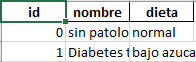
\includegraphics[scale=1]{BasePatologias} 
\caption{Estructura base de datos Patologías}
\end{figure}

\textbf{\textsc{Registro}}\\
Base de datos que se encuentra en la ruta: assets/RegistroMejora.xlsx, y se encarga de llevar un registro de la mejora del usuario en la aplicación. Esta base de datos guarda los datos imprescindibles para el ajuste de la formula del TMB respecto al usuario concreto.\\
En el momento que un usuario se registra, tiene tres posibilidades de tipo de dieta:
\begin{enumerate}
\item \textbf{bajar:} Se crea un valor inicial igual a -400
\item \textbf{Mantener:} Se crea un valor inicial igual a 10
\item \textbf{Subir:} Se crea un valor inicial igual a 400. 
\end{enumerate}
El valor inicial a la hora del registro, es el suplemento que se añade al resultado de la formula del metabolismo basal, para que las calorias a ingerir por el usuario sean las necesarias para lograr el objetivo que se ha propuesto a través del tipo de dieta. Mantener tiene un valor inicial a 10, porque en caso de tener que reajustarse.
Esta base de datos se estructura de la siguiente manera:
\begin{figure}[htb]
\centering
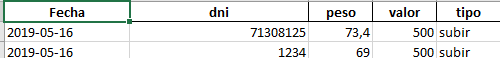
\includegraphics[scale=1]{registroMejora} 
\caption{Estructura base de datos Registro}
\end{figure}
Esto se debe a:
\begin{enumerate}
\item \textbf{Fecha:} Guarda la ultima vez que se edito la información. De esta manera se puede calcular el peso que se debería haber progresado hasta dicha fecha. No admite cambios de menos de una semana, pues el resultado podría alterar el ajuste del valor.
\item \textbf{dni:} DNI del usuario para saber de quien es el registro que se esta llevando.
\item \textbf{Peso:} El peso de la ultima vez que el usuario edito la información respectiva a su peso. Esto ayuda al seguimiento de la dieta y sus objetivos.
\item \textbf{Valor:} Valor que mas tarde se suma al calculo TMB y que ayuda a cumplimentar mejor su objetivo.
\item \textbf{tipo:} Tipo de dieta u objetivo de la dieta del usuario. Sirve para saber si el usuario a cambiado de objetivo y en caso de no hacerlo, ver como va el progreso del usuario.
\end{enumerate}
\subsubsection{Guardar Todo}
Función que se encarga de juntar en una única función el almacenamiento de todos los datos con los que se trabaja en esta herramienta. Dentro de esta función encontramos:
\begin{itemize}
\item	\textbf{guardarHistorial:} Como el propio nombre indica, se encarga de almacenar las selecciones que hicimos en el mismo día en la base de datos. A través de la librería dateTime de Python sacamos el día de hoy, con la fecha en forma de cadena de caracteres y el DNI del usuario creamos la clave primaria, no se puede repetir dos veces esta combinación, si a la hora de guardar ya existe, se actualiza pero no se añade; se crea un objeto tipo DataFrame segregado del array menuDeHoy, y se escribe en el Excel “historial”.
\item	\textbf{guardarUsuario:} Mencionada en el apartado anterior, se encarga de guardar el groso de la aplicación, que es todos los cambios que hayas hechos en la aplicación respecto a la comida permitiendo que el programa poco a poco se vaya adecuando a los gustos y lo que mas come el usuario.
\item	\textbf{guardarDatos:} Guarda los datos del usuario. Se llama en dos ocasiones, cuando se guarda todo y cuando se edita la información del usuario. La primera vez, en la ocasión que se guarda todo, es redundante, se hace para tener un respaldo en caso de que al editar usuario se de algún fallo y no se guarde, en un principio, en el momento que edites la información del usuario y se pulse en “Aceptar y guardar”, se guardarían los datos.
\end{itemize}

\subsubsection{getXXXX}
En este apartado se respaldaran las tres funciones que se encargan de dar la información de una fila concreta de una de las colecciones de la base de datos.
\subsection{Vista}
Para empezar, recordar que se ha seguido una adaptación de la estructura  típico MVC, donde se sustituye el modelo y el controlador propio y se tiene una vista adaptada, esto ya fue explicado al inicio de este apartado, a continuación me centrare en la vista.\\

En el módulo vista se muestran, o llevan a cabo toda función que tendrá influencia en lo que el usuario ve, es decir, actualización de pantallas, muestra de datos, transacciones entre las dos ventanas principales, el cambio de los gráficos, etc.\\

El modulo vista contiene tres variables calves globales, que son el DNI del usuario (usr), la contraseña del usuario (contraseña) y la bandera. De los dos primeros poco hay que explicar, pero del ultimo sí, esto se hará en el siguiente apartado, junto a la debida explicación de las funciones que hacen uso de ello.\\
\subsubsection{Comprobación usuario}
Empezando por la función “cambio”, que se nombro de esta manera porque indica un cambio en la funcionalidad del programa, explicamos esto:\\
El programa sigue su curso, cuando se cierra la ventana de log-in, o acceso, según como se haya procesado la información en cambio cuando la ventana se cierra, el programa continúa con su normal ejecución o se cierra completamente.\\

Cambio comprueba que la combinación usuario y contraseña sea válida en caso de ser así cambia el valor de bandera a verdadero (True), indicando así que el acceso a sido un éxito, si no, la bandera seguirá a False, y se mostrara por pantalla un mensaje de error.\\

Cuando la tupla usuario y contraseña es validad cierra la pantalla de “log-in”, lo que hace que en el “main” se siga con su normal ejecución, lo cual lleva, de manera directa a una condición que comprueba que la bandera es verdadera, si lo es relanza la aplicación principal, sino cierra el programa, y se termina toda ejecución.\\

Como el propio nombre indica getBandera devuelve este valior al main.\\

\subsubsection{Seleccionar y refrescar}
Sin duda alguna esto presento uno de los mayores retos de la aplicación debido a las deficiencias que presenta Python para construir interfaces gráficas, y dentro de dichas deficiencias generales, se añadía la dificultad que presentaba el simplismo de la librería tkinter para dichas interfaces.\\

Todo surgió de la necesidad de actualizar lo que se mostraba por pantalla cada vez que hacía una elección, pues si se quería sacar de este proyecto la mayor precisión posible del sistema de recomendación, cada elección, cada cambio de variable, debía suponer nuevas recomendaciones, esto en un principio parecía sencillo, pero Tkinter no permite la recarga de los datos, sino que al inicio del programa lo “dibuja”, todo de manera simultánea, impidiendo una actualización del frame cada vez que haya un cambio, por ello se crearon una serie de funciones, necesarias las cuales se engloban en una mayor, para que de una llamada realice todas las funciones necesarias.\textbf{seleccionarYActualizarResto}, esta función se encarga principalmente de actualizar todos los datos en pantalla, el menú que hemos comido hoy, ademñas de llamar a la función  \textbf{seleccionar}, la cual guarda la opción escogida y bloquea las posibles opciones, y acto seguido recorre las otros cuatro frames recalculando todas las listas, todas los resultados y sus respectivos LRE, etc. \\

Se ha decidido que para evitar errores de coherencia el programa solo actualizará aquellos frames no bloqueados por el método seleccionar, sacrificando un pequeño porcentaje de la precisión, para conseguir un funcionamiento mas fluido sin errores de compatibilidad o múltiples selecciones.\\
\subsection{Main}
Es la columna vertebral del programa, el cual, se encarga de cargar y procesar toda la información relevante que más adelante se va a ir editando en el programa, el main tiene una única función y el resto se divide en clases que se instancian en esta función.\\

La función principal hace de flujo de entrada y salida, donde un if condicional hace la función de interruptor permitiendo que la aplicación original, distribuida en clases se lance, o se cierre, como se ha explicado anteriormente.\\

Todo se basa en una especie de jerarquía de objetos, en el que el objeto principal (Menú principal), contiene otros tres objetos que estos a su vez contienen otros tantos, creando una simple estructura de árbol, entendible por cualquier programador. \\

De entre las tres subclases, instanciadas dentro del Menú principal (Usuario, Dieta, Historial), cabe destacar la de Dieta, pues esta a su ver tiene una clase por cada comida, estas clases son actualizadas constantemente en cuanto se hace algún cambio en el programa, esto es una abstracción del \textbf{ patrón de diseño observador}, en el que las clases observan esperando el cambio para actualizar sus recomendaciones.\\

Se quiso evitar un main lioso con cosas que no son propias del dicho, por ello se separo en lo que es el main, y las clases las cuales, se encargan del funcionamiento principal del programa. De alguna forma, podríamos ver el main como los cimientos del programa completo, y los diferentes módulos, son los encargados de terminar de construir el programa.
\section{Herramientas}
Una vez explicadas el por que de cada decisión que se ha tomado a lo largo del desarrollo del programa, y expuesto cada decisión meticulosamente, procurando que cualquier duda del lector respecto a como se ha trabajado quede resuelta; Nos centraremos en mencionar de manera breve, dando una ligera explicación del por qué, se han usado las herramientas que se han usado para el desarrollo del programa.
\subsubsection{Anaconda}
Distribución de código abierto, la cual, esta indicada para el análisis, procesamiento y computo de datos, de Python y R, trae consigo una serie de programas y características entre los que destacaremos: Spyder y VisualCode.\\

Sobre la razón, por la cual, se decidió usar anaconda es básica, la propia definición lo dice, a fin de cuentas, es una distribución para el análisis de datos con Python y R, lo cual, es de manera encubierta, el principal trabajo en este proyecto.
\subsubsection{VisualCode}
Al igual que Spyder, es un entorno de desarrollo incluido en el paquete de anaconda, con la diferencia de que VisualCode, es ampliamente utilizado por la comunidad de programadores para múltiples lenguajes, y frameworks, como angular2, javascript, c3, Python, ect.\\

Se pensó largo y tendido sobre que entorno utilizar entre Spyder y VisualCode, y durante los primeros periodos de la aplicación, se turnaron ambos sin ninguna razón aparante, con el tiempo, me sentí más cómodo trabajando con Spyder, y lo fui adoptando como entorno principal, delegando en VisualCode la tarea de hacer debug, debido a la notable mejora que este presenta sobre Spyder.\\

Indicar que antes de empezar se probaron varios entornos como NoteBook, PyCharm, y eclipse añadiendo el API de Python, pero se acabo decantando por estas dos herramientas nombradas anteriormente.\\

\subsubsection{GitHub}
Proyección de la metodología GIT para el almacenamiento y control de versiones, sin duda GIT es actualmente la estructura más usada en el mundo de la programación, y GitHub, una de las herramientas más conocidas y valoradas que hay.  Con el tiempo, fue mi mayor aliado, permitiéndome recuperar antiguas versiones con el programa era corrompido por algún error lógico, y dando una seguridad de soporte sobre el desarrollo del proyecto.
\subsubsection{GitKraken}
Potente interfaz gráfica multiplataforma desarrollada por Electron, que nos permite controlar de forma sencilla y cómoda nuestro repositorio GitHub, permitiendo que el uso y control del GitHub fuera más ameno y rápido, sin duda es una de las mejores aplicaciones que he probado, y de las que mas me han ayudado a lo largo del proyecto.


